%!TEX encoding = UTF-8 Unicode
%!TEX root = ../galgas-book.tex

%--------------------------------------------------------------
\chapterLabel{Projet \texttt{Xcode} et application Cocoa}{appliCocoa}
%-------------------------------------------------------------

\tableDesMatieresLocaleDeProfondeurRelative{1}


Vous pouvez demander à GALGAS d'engendrer un projet \texttt{Xcode}, qui contiendra~:
\begin{itemize}
  \item le compilateur en version \emph{release} sous la forme d'un utilitaire en ligne de commande~; 
  \item le compilateur en version \emph{debug} sous la forme d'un utilitaire en ligne de commande~; 
  \item une application Cocoa permettant d'appeler les deux utilitaires.
\end{itemize}






\sectionLabel{Paramétrage du projet GALGAS}{parametrageProjetGALGAS}

Pour engendrer un projet \texttt{Xcode}, il y a deux attributs obligatoires, et un attribut optionnel~:
\begin{itemize}
\item un premier attribut obligatoire qui définit le OSX SDK et la version système cible (\refSubsectionPage{attributOSXSDK})~;
\item un second attribut obligatoire \ggs=%applicationBundleBase= (\refSubsectionPage{attributapplicationBundleBase})~;
\item un attribut optionnel \ggs=%macCodeSign=, qui définit comment est signé l'application OS X engendrée (\refSubsectionPage{attributmacCodeSign}).
\end{itemize}




\subsectionLabel{Attribut définissant le OSX SDK et la version système cible}{attributOSXSDK}

Pour engendrer un projet \texttt{Xcode}, il vous suffit d'ajouter une déclaration telle que \ggs+%MacOS+ dans votre fichier projet (d'extension \tpp{.galgasProject}, voir \refChapterPage{composantProjet}). Par exemple~:

\begin{galgas}
project (0:0:1) -> "logo" {
  %applicationBundleBase : "fr.what"
  ...
\end{galgas}

%Vous pouvez aussi utiliser l'option \texttt{-{-}macosx=$n$} (\refSectionPage{optionsGeneration}). Attention, cette option ne vous dispense pas de préciser \ggs=%applicationBundleBase=.
%
%Un projet \texttt{Xcode} définit la version de Mac OS pour laquelle il va être compilé~: ainsi, \ggs+%Lion+ définit la version \texttt{Lion} (10.7). Le \refTableau{options-pour-xcode} liste les différents options possibles. GALGAS fixe la version indiquée dans le projet \texttt{Xcode}, et il faut ensuite que la version de \texttt{Xcode} utilisée soit compatible avec ce réglage. L'option \ggs+%LatestMacOS+ correspond au réglage correspondant du projet \texttt{Xcode} engendré. Quand \ggs+%SnowLeopard+ est sélectionné, l'application Cocoa engendrée utilise le \emph{garbage collector}. Sinon, elle adopte l'\emph{Automatic Reference Counting} (\emph{ARC}).

%
%\begin{table}[!t]
%  \centering
%  \begin{tabular}{rlll}
%    \textbf{Option} & \textbf{Version SDK Mac OS} & \textbf{Version de}  &  \textbf{Gestion mémoire}\\
%                    &                             & \textbf{déploiement} &                          \\
%    \ggs+%SnowLeopard+ & \texttt{SnowLeopard} (10.6) & 10.6  & \emph{Garbage Collector}\\
%    \ggs+%Lion+ & \texttt{Lion} (10.7) & 10.7 & \emph{ARC}\\
%    \ggs+%MountainLion+ & \texttt{Mountain Lion} (10.8) & 10.8 & \emph{ARC}\\
%    \ggs+%Mavericks+ & \texttt{Mavericks} (10.9) & 10.9 & \emph{ARC}\\
%    \ggs+%Yosemite+ & \texttt{Yosemite} (10.10) & 10.10  & \emph{ARC}\\
%    \ggs+%YosemiteElCapitan+ & \texttt{El Capitan} (10.11) & 10.10  & \emph{ARC}\\
%    \ggs+%ElCapitan+ & \texttt{El Capitan} (10.11) & 10.11  & \emph{ARC}\\
%    \ggs+%Sierra+ & \texttt{Sierra} (10.12) & 10.12  & \emph{ARC}\\
%    \ggs+%ElCapitanSierra+ & \texttt{Sierra} (10.12) & 10.11  & \emph{ARC}\\
%    \ggs+%LatestMacOS+ & -- & -- & --\\
%  \end{tabular}
%  \caption{Options du projet GALGAS indiquant la version Mac OS}
%  \labelTableau{options-pour-xcode}
%\end{table}





\subsectionLabel{Attribut \texttt{\%applicationBundleBase}}{attributapplicationBundleBase}\index{\%applicationBundleBase}

Il y a un second attribut obligatoire à ajouter dans le projet GALGAS~: \ggs+%applicationBundleBase+. Celle-ci fixe le \emph{Bundle Identifier} de l'application Cocoa. À la chaîne définie dans l'option (ici \ggs+"fr.what"+) est ajouté le nom du projet (défini dans l'en-tête, ici \ggs+"logo"+), précédé par un point~: le \emph{Bundle Identifier} est donc \tpp{fr.what.logo}.


\subsectionLabel{Attribut \texttt{\%macCodeSign}}{attributmacCodeSign}\index{\%macCodeSign}

Par défaut, l'application engendrée par Xcode n'est pas signée. Cela signifie qu'elle tournera sur le système et la machine où elle a été compilée, mais peut-être pas sur un autre système et / ou une autre machine.

L'attribut \ggs=%macCodeSign= permet de préciser comment Xcode va signer l'application.

\fbox{\begin{minipage}{1.0\textwidth}
Dans la version actuelle de GALGAS, l'attribut \texttt{\%macCodeSign} permet de signer l'application avec votre compte \texttt{Mac Developer}, ou un certificat défini dans le \emph{Trousseau d'accès}, par exemple un certificat auto-signé.
\end{minipage}}

L'attribut \ggs=%macCodeSign= doit être associé à une chaîne de caractères, qui comprend deux éléments séparés par un «~:~»~:
\begin{galgas}
  %macCodeSign = "MacDeveloper:ZW8HY75J3X"
\end{galgas}
ou 
\begin{galgas}
  %macCodeSign = "Certificate:John Egg Smith"
\end{galgas}
Le premier correspond au certificat associé à votre compte \texttt{Mac Developer}, le second à un certificat détenu dans le \emph{Trousseau d'accès} («~\emph{Key Chain}~»).

\fbox{\begin{minipage}{1.0\textwidth}
Manifestement, Apple recommande de signer l'application par votre compte \texttt{Mac Developer} : l'interface de Xcode 8 ne permet pas de signer une application avec un certificat auto-signé, mais accepte un projet contenant cette signature.
\end{minipage}}

Les chaînes \tpp{ZW8HY75J3X} et \tpp{John Egg Smith} sont juste des exemples, il faut que vous utilisiez des valeurs valides.

Pour obtenir la chaîne associée à votre compte \texttt{Mac Developer}, vous avez plusieurs possibilités~:
\begin{itemize}
  \item utiliser l'utilitaire \texttt{certtool} (\refSubsubsectionPage{utilitaireCerttool})~;
  \item utiliser l'application \emph{Trousseaux d'accès} (\refSubsubsectionPage{appKeyChain})~;
  \item signer l'application dans le projet Xcode engendré, et observer sa description dans un éditeur de texte~: \refSubsubsectionPage{signatureDansXcode}.
\end{itemize}

La \refSubsubsectionPage{definirCertificatAutoSigne} montre comment définir un certificat auto-signé. 

Une fois que l'attribut \ggs=%macCodeSign= aura été défini, vous pourrez effectuer la compilation GALGAS de votre projet. Compiler le projet Xcode engendrera une application signée. On pourra le vérifier, comme expliqué à la \refSubsectionPage{verifierSignatureAppli}.

\subsubsectionLabel{Utilitaire \texttt{certtool}}{utilitaireCerttool}

Sur Mac OS X, l'utilitaire \texttt{certtool} permet de manipuler les certificats. L'option \texttt{y} permet de les afficher. Entrer dans le terminal~:
\begin{SHELL}
certtool y
\end{SHELL}
L'exécution de la commande affiche sur le terminal une grande quantité de lignes dans lesquelles il faut rechercher le certificat correspondant à votre compte  \texttt{Mac Developer}. On peut faciliter ce travail en redirigeant la sortie de la commande dans un fichier~: 
\begin{SHELL}
certtool y > certificats.txt
\end{SHELL}

Rechercher dans la sortie de la commande la chaîne \tpp{Mac Developer}. Vous la trouvez associée avec l'adresse électronique de votre compte développeur (ici \tpp{john@smith.nowhere})~:
\begin{SHELL}
Subject Name~~~~:\\
Other name~~~~~~: 9ZED6TWL8M\\
Common Name~~~~~: Mac Developer: john@smith.nowhere (Q933RG93DL)\\
OrgUnit~~~~~~~~~: ZW8HY75J3X\\
Org~~~~~~~~~~~~~: JOHN SMITH\\
Country~~~~~~~~~: US
\end{SHELL}

La chaîne recherchée apparaît associée à l'entrée \tpp{OrgUnit}.



\subsubsectionLabel{Application \emph{Trousseaux d'accès}}{appKeyChain}

L'application \emph{Trousseaux d'accès} (« Keychain Access ») permet de retrouver les certificats~; ouvrir l'application, sélectionner dans la barre latérale \tpp{Mes certificats}, et, éventuellement, entrer \tpp{Mac Developer} dans la zone recherche. Le certificat recherché doit apparaître comme l'indique la \refFigure{}{figureAppliTrousseauxAccess}. Double-cliquer pour en avoir le détail~: \refFigure{}{figureDetailCertificat}. La chaîne recherchée apparaît associée à l'entrée \tpp{Unité d'organisation}.


\begin{figure}[!t]
  \centering
  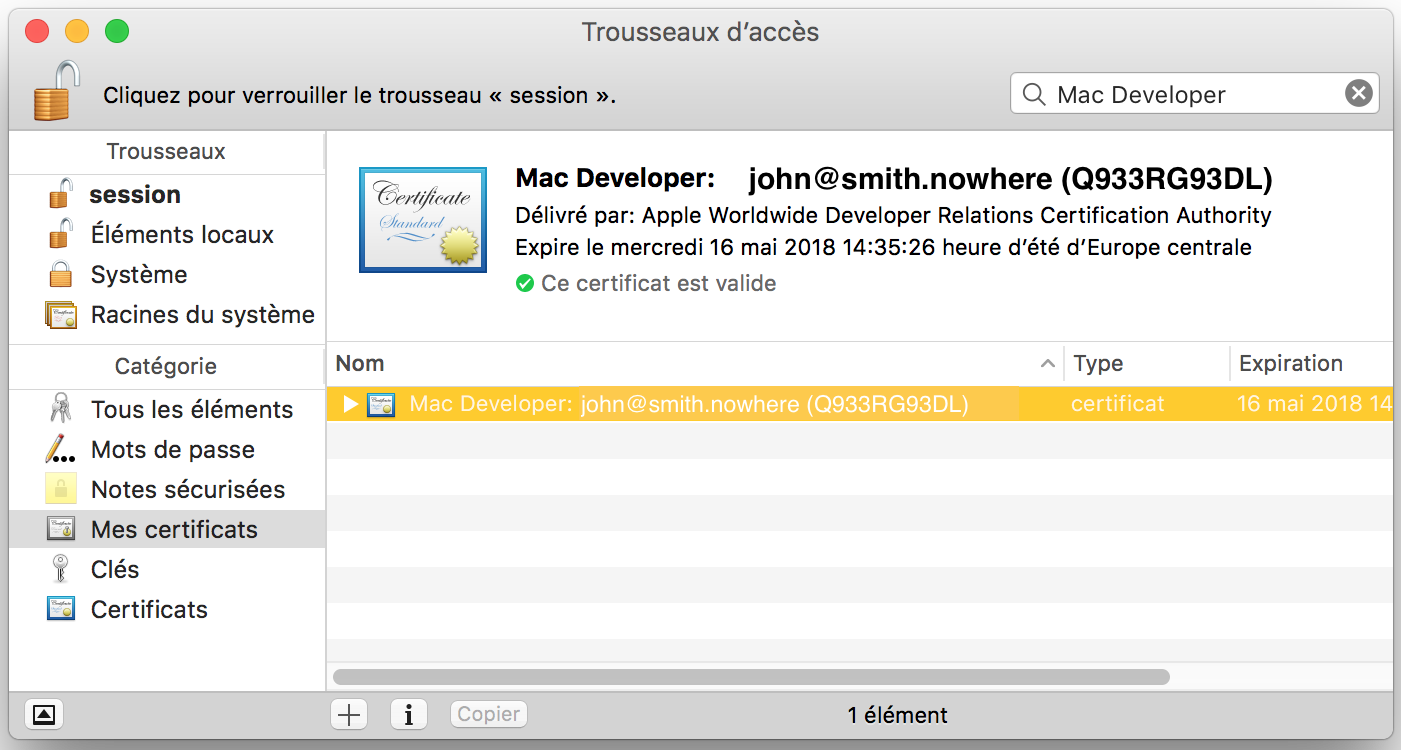
\includegraphics[width=14cm]{chapitre-cocoa-features/trousseaux-acces.png}
  \caption{Application \emph{Trousseaux d'accès}}
  \labelFigure{figureAppliTrousseauxAccess}
\end{figure}




\begin{figure}[!t]
  \centering
  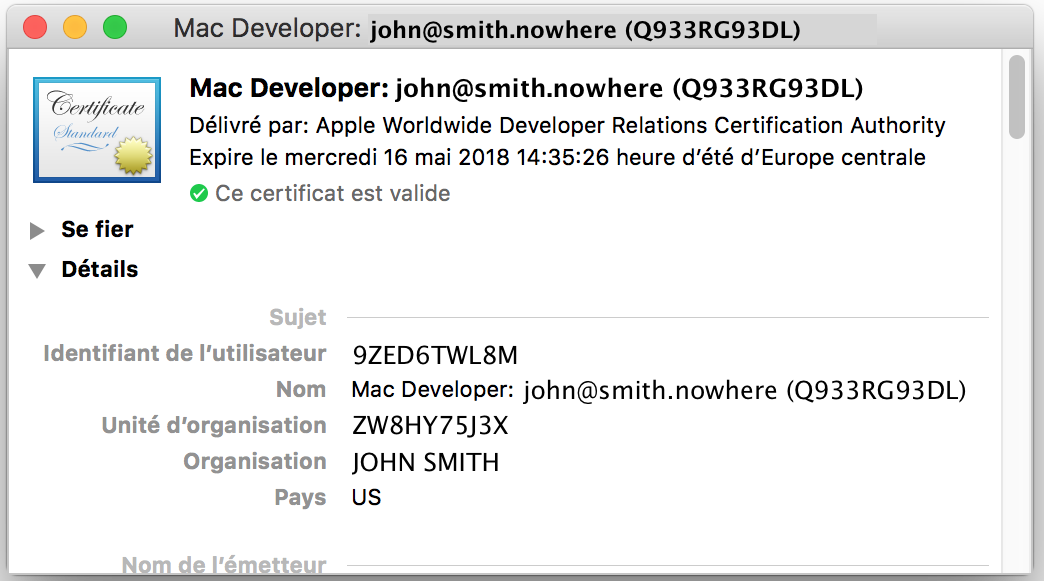
\includegraphics[width=14cm]{chapitre-cocoa-features/certificat.png}
  \caption{Détail du certificat}
  \labelFigure{figureDetailCertificat}
\end{figure}






\subsubsectionLabel{Signature dans Xcode}{signatureDansXcode}

On peut utiler Xcode pour retrouver la chaîne recherchée. Pour cela, on va modifier le projet Xcode engendré pour signer l'application engendrée. 

\fbox{\begin{minipage}{1.0\textwidth}
Évidemment, toute modification de Xcode pourra être écrasée par une recompilation GALGAS du projet : on n'utilise donc la modification du projet juste pour découvrir la chaîne recherchée.
\end{minipage}}




\begin{figure}[!t]
  \centering
  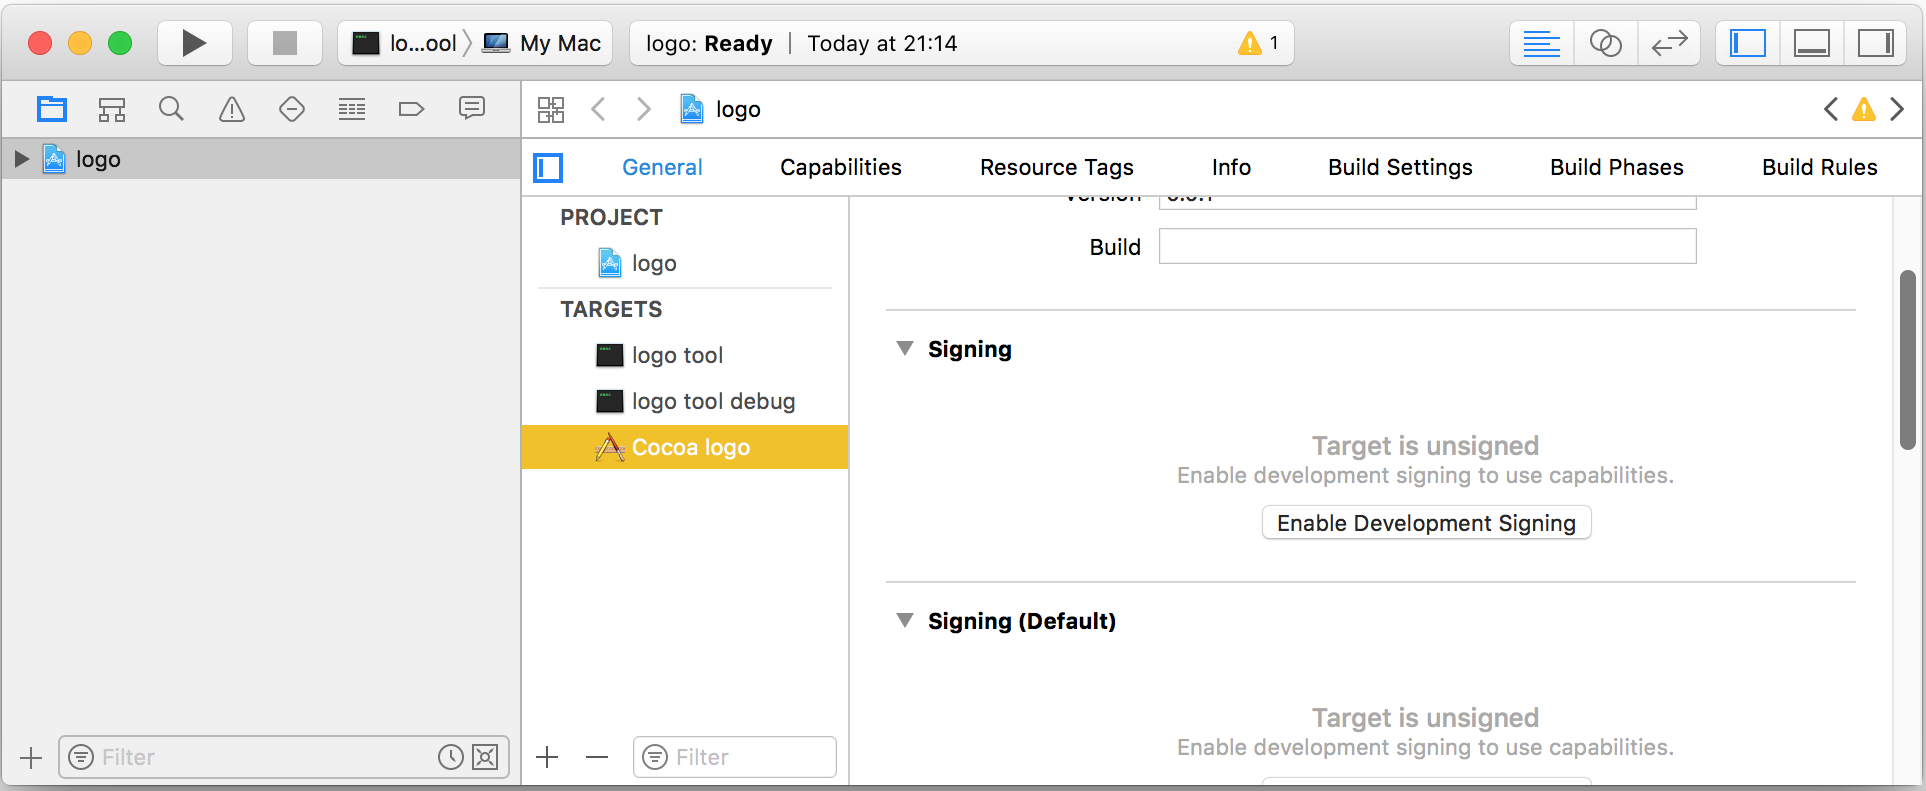
\includegraphics[width=15cm]{chapitre-cocoa-features/projet-xcode-sans-signature.png}
  \caption{Projet \texttt{Xcode} sans signature}
  \labelFigure{figureXcodeSansSignature}
\end{figure}


\begin{figure}[!t]
  \centering
  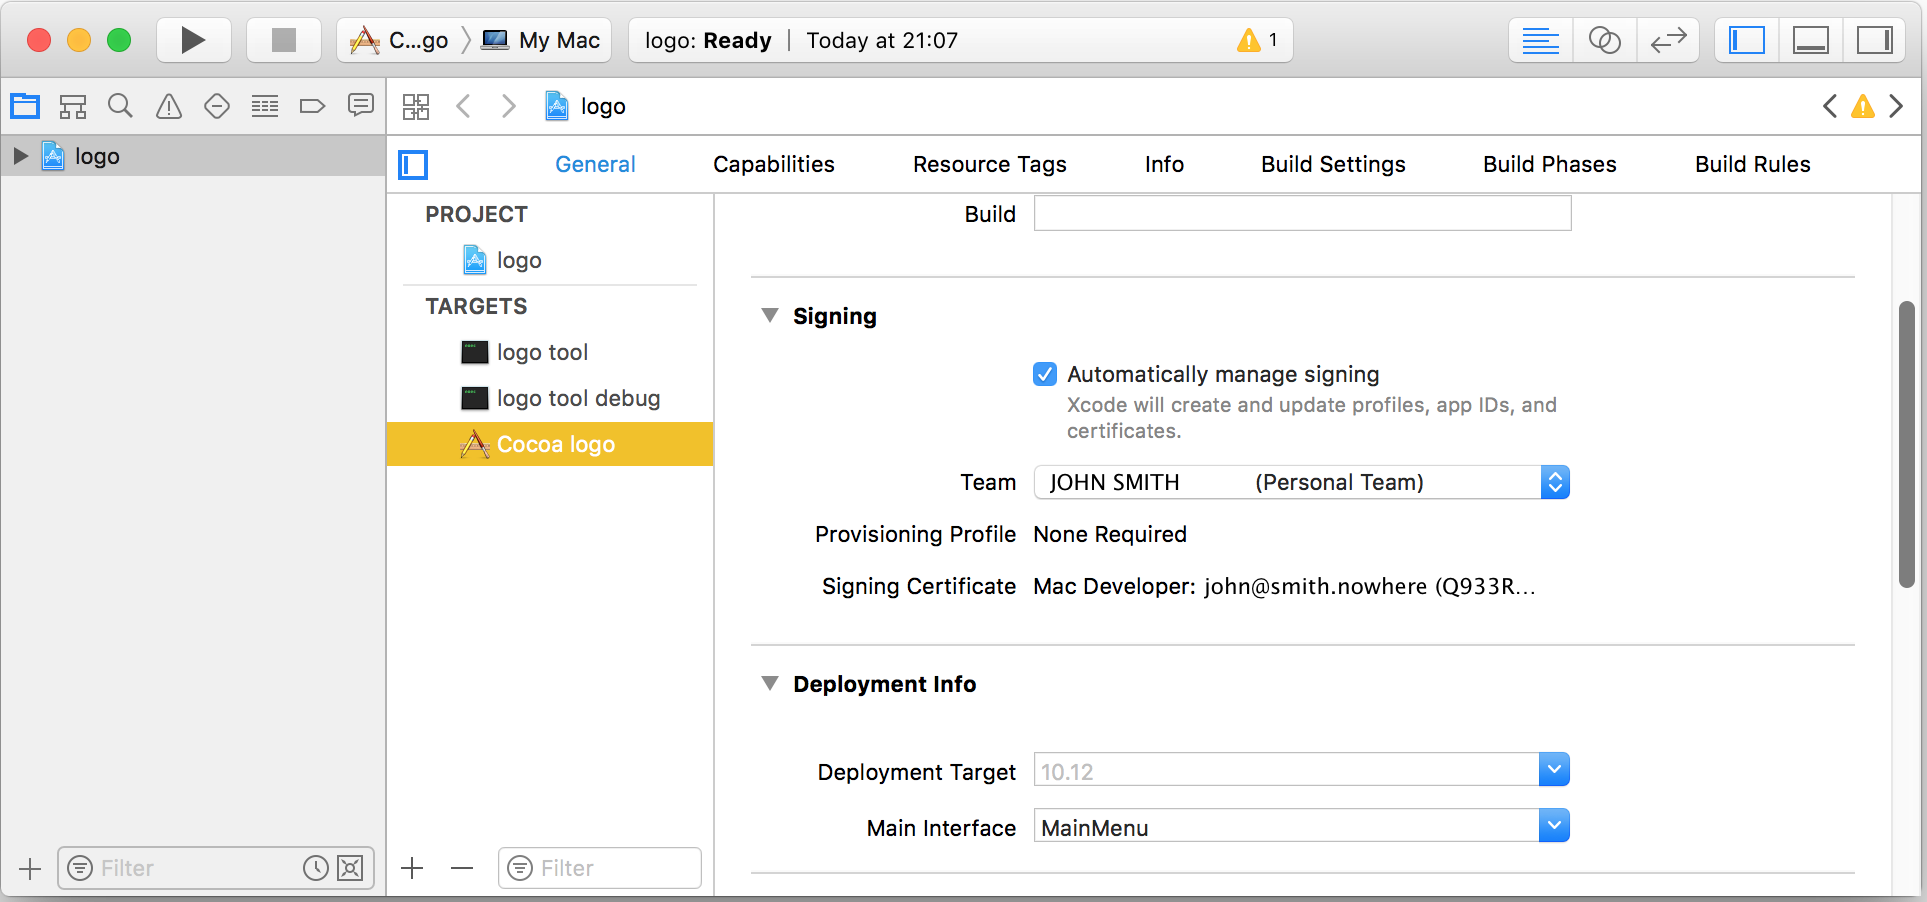
\includegraphics[width=15cm]{chapitre-cocoa-features/projet-xcode-avec-signature.png}
  \caption{Signature à partir du projet \texttt{Xcode}}
  \labelFigure{figureSignatureXcode}
\end{figure}

Ouvrir donc le projet Xcode, sélectionner \tpp{logo} dans la barre latérale gauche, puis la cible (dans «~TARGETS~») \tpp{Cocoa logo}, puis l'onglet \tpp{General}, et repérer le bloc \tpp{Signing}~: \refFigure{}{figureXcodeSansSignature}. Cliquez alors sur «~Enable Development Signing~», de façon à aboutir à la \refFigure{}{figureSignatureXcode}. 

Maintenant, fermer Xcode. Le fichier projet Xcode \tpp{logo.xcodeproj} est en fait un répertoire. Pour afficher son contenu, effectuer un clic secondaire sur l'icône de \tpp{logo.xcodeproj}, et sélectionner dans le menu contextuel qui apparaît l'item «~\emph{Afficher le contenu du paquet}~» (\refFigure{a}{figureOuverturePaquetXcode})~; la fenêtre qui apparaît (\refFigure{b}{figureOuverturePaquetXcode}) montre le contenu de paquet. Le fichier qui nous intéresse est \tpp{project.pbxproj}. Ce fichier est un fichier texte seul, ouvrez-le avec un éditeur de texte. Repérer la ligne définissant le paramètre \tpp{DEVELOPMENT\_TEAM}~:
\begin{SHELL}
DEVELOPMENT\_TEAM = ZW8HY75J3X;
\end{SHELL}
La valeur associée au paramètre \tpp{DEVELOPMENT\_TEAM} est la chaîne recherchée~: \texttt{ZW8HY75J3X}.

\begin{figure}[!t]
  \centering
  \subfloat[Afficher le contenu du paquet]{
   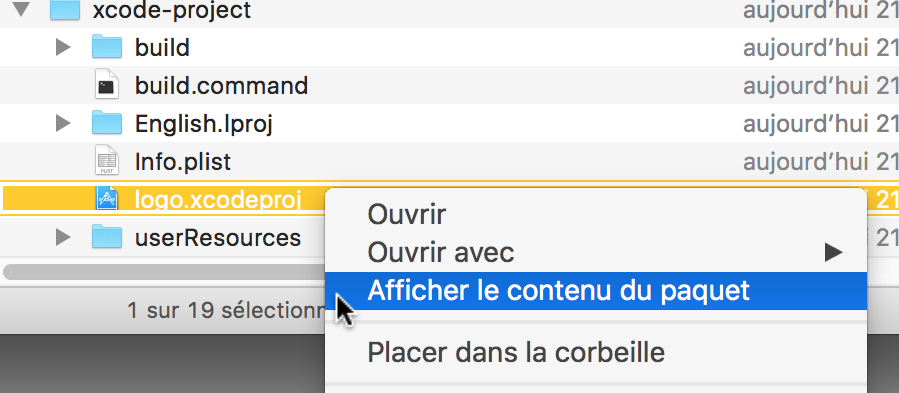
\includegraphics[width=8cm]{chapitre-cocoa-features/ouverture-paquet-xcode.png}
  }
  \hspace{1 cm}
  \subfloat[Contenu du paquet]{
   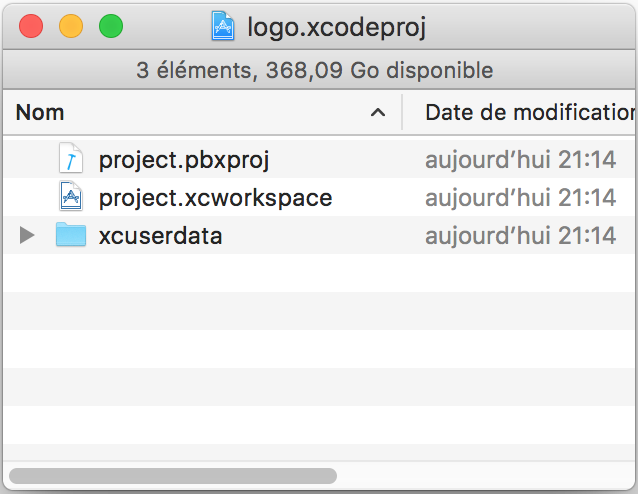
\includegraphics[width=5cm]{chapitre-cocoa-features/contenu-paquet-xcode.png}
  }
  \caption{Afficher dans le Finder le contenu du paquet projet Xcode}
  \labelFigure{figureOuverturePaquetXcode}
\end{figure}






\subsubsectionLabel{Définir un certificat auto-signé}{definirCertificatAutoSigne}

Pour définir un certificat auto-signé, appler l'application «~\emph{Trousseaux d'accès}~» («~\emph{Keychain Access}~»). Ensuite, sélectionner dans le menu de l'application \tpp{Assistant de certification} -> \tpp{Créer un certificat…}, comme indiqué à la \refFigure{a}{figureDefinirCertificatAutoSigne}. Ensuite, dans la fenêtre qui apparaît (\refFigure{b}{figureDefinirCertificatAutoSigne}), entrer le nom que vous allez donner au certificat (ici «~John Egg Smith~»), sélectionner pour le \tpp{Type d'identité} «~Racine auto-signée~», et pour \tpp{Type de certificat} «~Signature de code~». Terminer la création en cliquant sur \tpp{Créer}.

Le nom que vous avez donné au certificat est important, c'est lui que vous allez utilisez pour l'attribut \ggs=%macCodeSign= (respecter absolument la casse et les espaces)~:
\begin{galgas}
  %macCodeSign = "Certificate:John Egg Smith"
\end{galgas}


\begin{figure}[!t]
  \centering
  \subfloat[Menu de création d'un certificat]{
   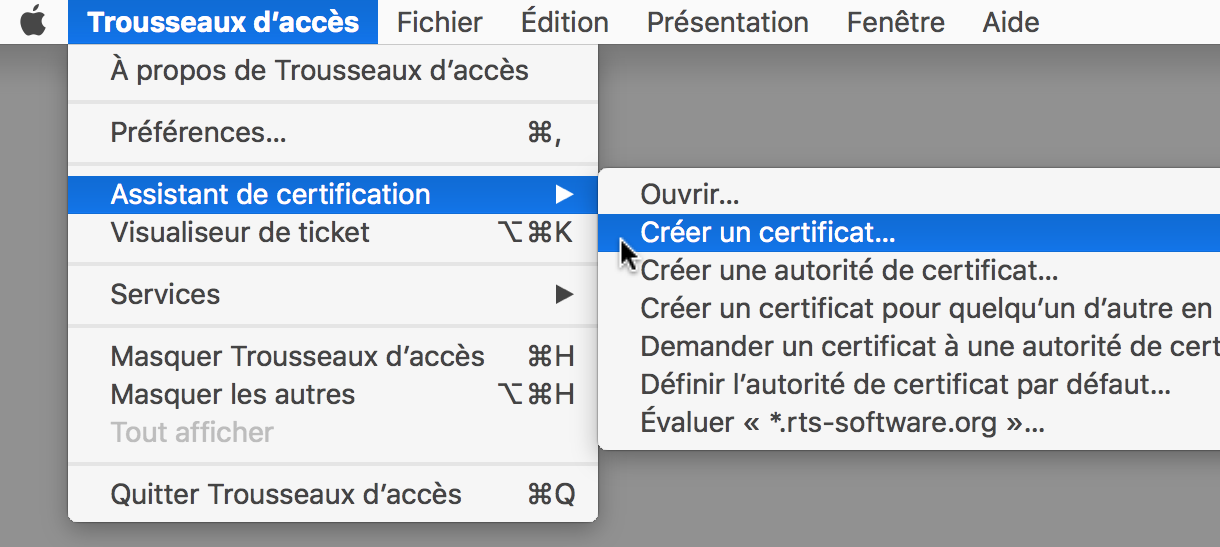
\includegraphics[width=7cm]{chapitre-cocoa-features/menu-creation-certificat.png}
  }
  \hspace{0.5cm}
  \subfloat[Création d'un certificat auto-signé]{
   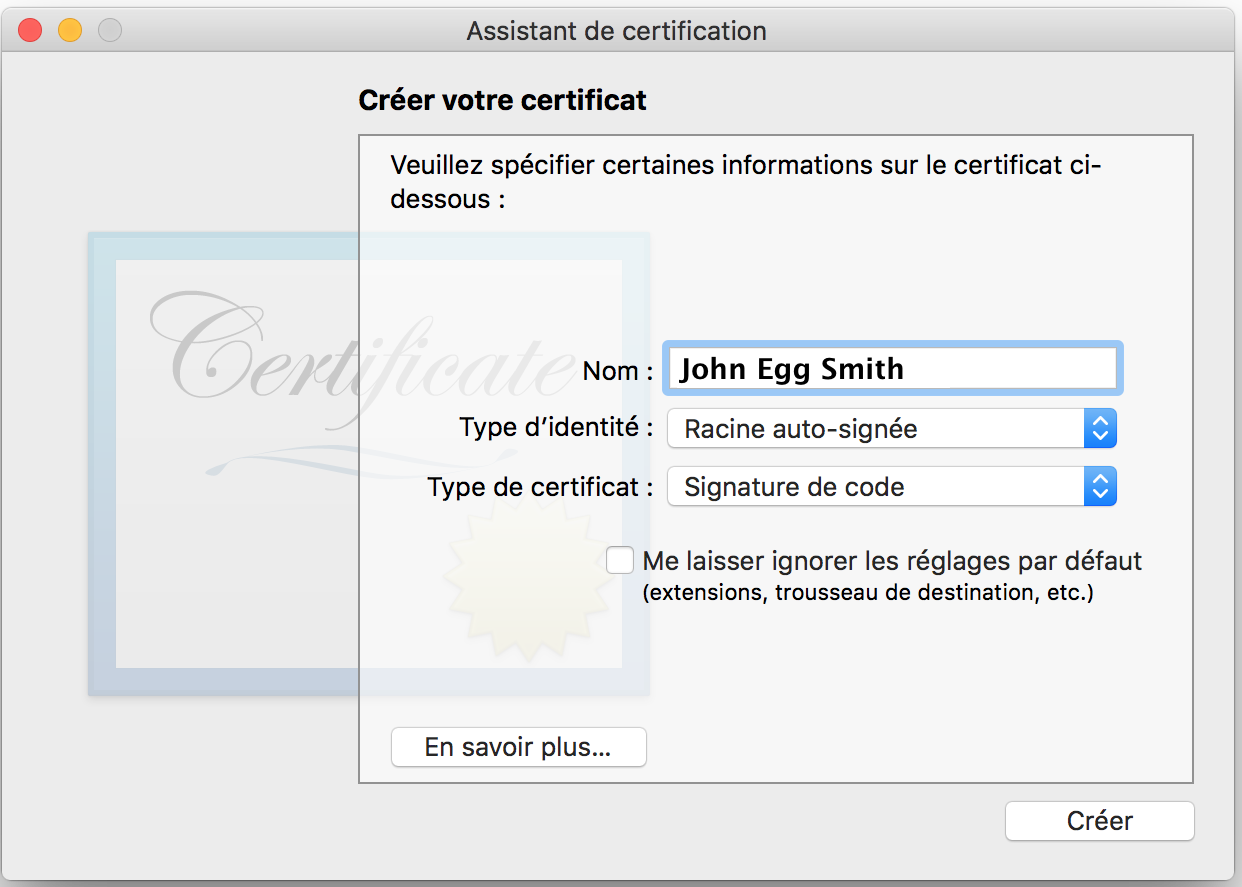
\includegraphics[width=7cm]{chapitre-cocoa-features/creation-certificat-autosigne.png}
  }
  \caption{Certificat auto-signé}
  \labelFigure{figureDefinirCertificatAutoSigne}
\end{figure}





\subsectionLabel{Vérifier la signature d'une application}{verifierSignatureAppli}

Pour vérifier la signature d'une application, on peut utiliser l'outil \tpp{spctl}. Dans le terminal, exécutez~:
\begin{SHELL}
spctl -a -t exec -vv \emph{chemin.app}
\end{SHELL}

Où \tpp{chemin.app} est le chemin vers l'application que la compilation du projet Xcode a créé.

Si l'application a été signée par le compte \texttt{Mac Developer}, l'exécution de la commande affiche~:

\begin{SHELL}
\emph{chemin.app}: accepted\\
override=security disabled\\
origin=Mac Developer: john@smith.nowhere (Q933RG93DL)
\end{SHELL}


Si l'application a été signée par un certificat auto-signé, l'exécution de la commande affiche~:

\begin{SHELL}
\emph{chemin.app}: accepted\\
override=security disabled\\
origin=John Egg Smith
\end{SHELL}


Si l'application n'a pas été signée, l'exécution de la commande~:
\begin{SHELL}
\emph{chemin.app}: accepted\\
source=no usable signature\\
override=security disabled
\end{SHELL}









\section{Projet \texttt{Xcode} engendré}


Quand le projet GALGAS est compilé, un répertoire \tpp{xcode-project} directory est créé, et contient~:
\begin{itemize}
\item le fichier projet \texttt{Xcode} ;
\item un fichier \tpp{build.command} ;
\item un fichier \tpp{Info.plist} ;
\item un répertoire \tpp{English.lproj} ;
\item un répertoire \tpp{userResources}.
\end{itemize}

Le rôle de chacun est précisé par le \refTableau{fichiers-repertoires-xcode}. Ne pas modifier ces fichiers et répertoires à la main, une compilation GALGAS supprimerait vos changements. La seule exception est le contenu du répertoire \tpp{userResources} qui n'est pas modifié par les compilations GALGAS.

\begin{table}[!t]
  \centering
  \begin{tabular}{rp{10cm}}
    \textbf{Fichier ou répertoire} & \textbf{Rôle}\\
    \tpp{build.command} & Effectue la compilation Xcode, appelable via une commande \emph{Shell} \\
    \tpp{Info.plist}    & Informations pour l'application Cocoa \\
    \tpp{English.lproj} & Informations pour l'application Cocoa \\
    \tpp{userResources} & Permet d'associer des icônes aux fichiers sources de votre compilateur, ainsi qu'à l'application Cocoa engendrée (voir \refSectionPage{ajouterIconesAppliCocoa}) \\
  \end{tabular}
  \caption{Fichiers et répertoires relatifs au projet Xcode}
  \labelTableau{fichiers-repertoires-xcode}
\end{table}





\sectionLabel{Définir des icônes pour votre application Cocoa}{ajouterIconesAppliCocoa}

Vous pouvez définir~:
\begin{itemize}
  \item une icône pour l'application Cocoa ;
  \item une icône particulière pour chaque type de fichier source.
\end{itemize}

Le nom de chaque fichier d'icône fixe son rôle~:
\begin{itemize}
  \item pour l'application Cocoa, le fichier d'icône doit s'appeler \tpp{application\_icns.icns}~;
  \item pour chaque type de fichier source, le nom est basé sur l'extension du fichier~: si celui-ci est par exemple \tpp{.logo}, le fichier d'icônes doit s'appeler \tpp{logo\_icns.icns}.
\end{itemize}

Ces fichiers d'icônes doivent être placés dans le répertoire \tpp{userResources}, et il faut ensuite refaire une compilation GALGAS pour que ces fichiers soient ajoutés au projet \texttt{Xcode}.

En résumé~:
\begin{enumerate}
  \item concevoir les fichiers d'icônes, en fixant leur nom comme indiqué ci-dessus ;
  \item placer ces icônes dans le répertoire \tpp{userResources} ;
  \item effectuer une compilation GALGAS~: celle-ci met à jour le projet \texttt{Xcode}, en ajoutant les fichiers d'icônes au \emph{target} Cocoa ;
  \item recompiler le \emph{target} Cocoa du projet \texttt{Xcode}~: les icônes sont prises en compte.
\end{enumerate}













\sectionLabel{Indexation des fichiers sources}{indexingYourSourceFiles}

Vous pouvez configurer votre projet GALGAS pour que l'application Cocoa engendrée établisse une indexation et des références croisées : un \tpp{cmd-click} affiche un menu contextuel. Cette indexation est basée sur l'analyse syntaxique. C'est ce qui a été fait pour l'application \texttt{CocoaGalgas} (\refFigurePage{}{indexingUnderCocoaGALGAS}). On voit dans le menu contextuel trois classes d'index : \tpp{Class Definition}, \tpp{Class Reference as Superclass} et \tpp{Abstract Category Method Definition}~; au dessous, les références croisées correspondantes.


%You can configure your project for enabling cross-referencing entities with your Cocoa application. This has been done in GALGAS, providing such feature (\refFigure{}{indexingUnderCocoaGALGAS}). The contextual menu is displayed with a \texttt{cmd-click}.

\begin{figure}[!t]
  \centering
  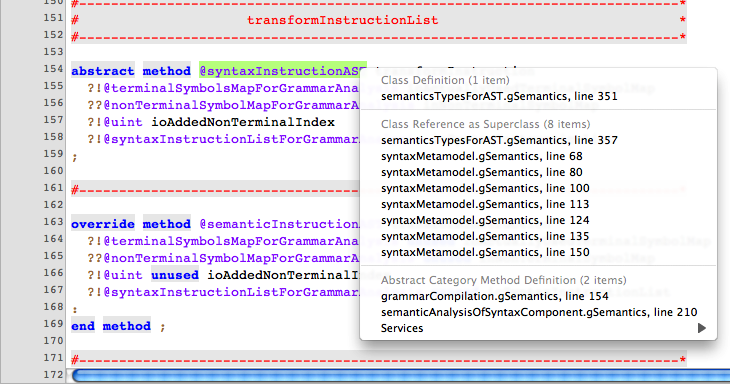
\includegraphics[width=14cm]{chapitre-cocoa-features/indexing-sample.png}
  \caption{Indexation et références croisées dans l'application CocoaGalgas}
  \labelFigure{indexingUnderCocoaGALGAS}
\end{figure}

Pour configurer votre projet, vous avez à modifier le composant \emph{lexique}, le composant \emph{syntax}, le composant \emph{grammar}, et la règle d'analyse du fichier source. Les cinq modifications sont présentées successivement ci-après, en prenant comme exemple le langage LOGO (\refSectionPage{presentation-logo}).





\subsection{En tête du composant \texttt{lexique}}

Il faut modifier l'en-tête, en ajoutant la déclaration  \ggs+indexing in+ :


\begin{galgas}
lexique logo_lexique indexing in "INDEXING" {
  ...
\end{galgas}

La chaîne \ggs+"INDEXING"+ définit le nom du répertoire qui contient les fichiers cache de l'indexation. Ce répertoire est relatif au répertoire qui contient le fichier source.

Note : si vous effectuez maintenant la compilation GALGAS, vous obtiendrez une erreur sur la définition de la grammaire, indiquant qu'elle doit aussi indiquer la prise en compte de l'indexation.




\subsection{En tête du composant \texttt{grammar}}

Il suffit de préfixer par \ggs+indexing+ l'en-tête du composant \ggs+grammar+ :

\begin{galgas}
indexing grammar logo_grammar ... {
  ...
\end{galgas}

Note : maintenant, la compilation GALGAS s'effectue sans erreur.




\subsection{Règle d'analyse des fichiers sources}

La règle d'analyse des fichiers source doit mentionner dans l'en-tête la grammaire utilisée pour l'analyse (pour l'exemple du langage LOGO, c'est le rôle de la troisième ligne \ggs+grammar logo_grammar+).

\begin{galgas}
case . "logo"
message "a source text file with the .logo extension"
grammar logo_grammar
?sourceFilePath:@lstring inSourceFile {
  grammar logo_grammar in inSourceFile
}
\end{galgas}

Quand le mode d'exécution (absence de l'option \tpp{-{}-mode}) est le mode par défaut, les instructions de la règle sont exécutées. Ci-dessus, la seule instruction est l'instruction \ggs+grammar logo_grammar in inSourceFile+ (ligne 5).

Quand le mode d'exécution (présence de l'option \tpp{-{}-mode}) n'est pas le mode par défaut, les instructions de la règle ne sont pas exécutées, et les opérations sont guidées par la grammaire indiquée ligne 3. Dans le cas de l'indexation, l'exécution construit l'indexation du fichier source.









\subsection{Déclaration des classes d'index}

La déclaration des classes d'index s'effectue dans l'analyseur lexical. Dans la cadre du langage d'exemple LOGO, on veut simplement indéxer les routines, plus précisément l'endroit de leur définition, et les endroits où elles sont appelées. On définit donc deux classes d'index \ggs+routineDefinition+ et \ggs+routineCall+. À chaque déclaration est associée une chaîne de caractères, qui sera le titre affiché dans le menu contextuel. 


\begin{galgas}
lexique logo_lexique indexing in "INDEXING" {
  ...
indexing routineDefinition : "Routine Definition"
  ...
indexing routineCall : "Routine call"
  ...
\end{galgas}


Ces définitions peuvent être placées à tout endroit dans la définition de l'analyseur lexical.








\subsection{Définition des entrées indexées}

L'analyseur syntaxique va être complété de façon à définir les symboles qui seront indéxés. Plus précisement, c'est l'instruction d'analyse de symbole terminal qui est modifiée.

Considérons d'abord la déclaration de routine. La règle de l'analyseur syntaxique qui définit cette analyse est :

\begin{galgas}
rule <routine_definition> {
  $ROUTINE$
  $identifier$ ?let routineName
  $BEGIN$
  <instruction_list>
  $END$
}
\end{galgas}

Le nom de la routine est défini par l'instruction \ggs+$identifier$ ?let routineName+ : on la modifie alors de façon à signifier que l'indentificateur doit être indéxé comme une définition de routine :

\begin{galgas}
rule <routine_definition> {
  $ROUTINE$
  $identifier$ ?let routineName indexing routineDefinition
  $BEGIN$
  <instruction_list>
  $END$
}
\end{galgas}

Maintenant, l'instruction d'appel de routine :

\begin{galgas}
rule <instruction> {
  select
    $CALL$
    $identifier$ ?let @lstring routineName
    $;$
  or
    ...
  end
}
\end{galgas}

On modifie de manière analogue l'instruction \ggs+$identifier$ ?let @lstring routineName+~:

\begin{galgas}
rule <instruction> {
  select
    $CALL$
    $identifier$ ?let @lstring routineName indexing routineCall
    $;$
  or
    ...
  end
}
\end{galgas}



\subsection{Compilation et essai}

Les modifications sont terminées. Vous pouvez recompiler votre projet (compilation GALGAS puis compilation de la cible Cocoa du projet \texttt{Xcode}). La \refFigure{}{exemple-indexation-logo} montre le résultat obtenu en effectuant un \tpp{cmd-click} sur le nom de la routine.

\begin{figure}[!t]
  \centering
  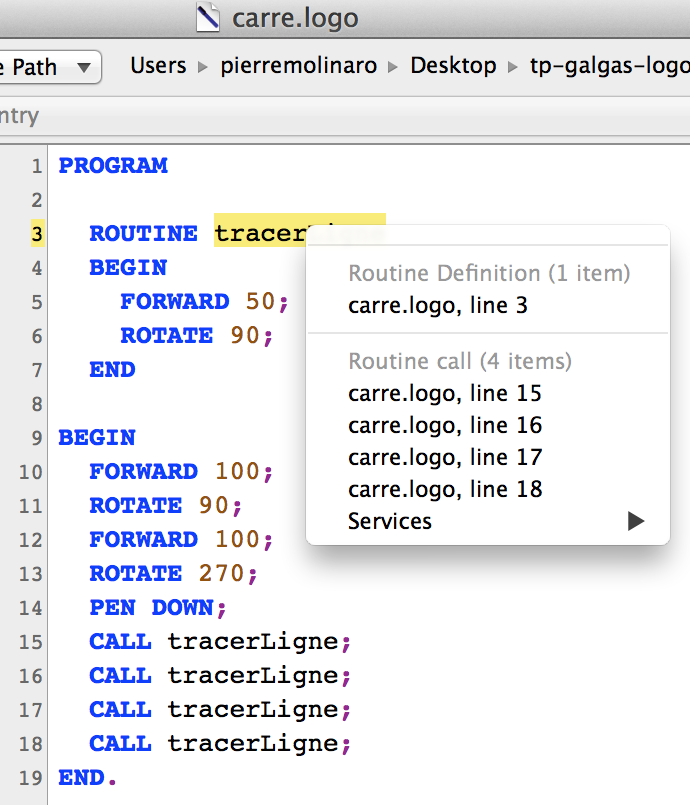
\includegraphics[width=8cm]{chapitre-cocoa-features/exemple-indexation-logo.png}
  \caption{Exemple d'indexation en LOGO}
  \labelFigure{exemple-indexation-logo}
\end{figure}



%\noindent{4} \textbf{Program component configuration.} Insert the \ggs+grammar+ declaration after the « \texttt{message ...} » declaration in every program rule concerned by indexing:
%
%\begin{galgas}
%case ...
%message ...
%grammar my_grammar
%?@lstring inSourceFile {
%  ...
%\end{galgas}
%
%
%
%
%
%
%\noindent{5} \textbf{Define indexing entries.} The indexing entries are defined within the rules of syntax components. The \emph{terminal check} instruction is the unique way for definition, by naming an index class name:
%
%\begin{galgas}
%syntax ... ("my_lexique.gLexique")~:
%  ...
%rule ... :
%  ...
%  $identifier$ ? ... indexing myIndexClass1 ;
%  ...
%end rule ;
%  ...
%\end{galgas}
%
%Any kind of terminal symbol accepts an « \texttt{indexing} » attribute : keywords, delimiters, literal string, integers, identifiers, \dots
%
%Several index class names can be named, using a comma as separator:
%\begin{galgas}
%  ...
%  $identifier$ ? ... indexing myIndexClass1, myIndexClass2 ;
%  ...
%\end{galgas}
%
%
%
%
%
%
%\noindent{6} \textbf{Compile and play.} Now, you can compile and run the Cocoa Application. With a \texttt{cmd}-click on an indexed terminal symbol, the contextual menu is displayed. You can delete the indexing directory at any moment, it will be rebuilt as needed.







